\section{Status of the analysis.}

To obtain the cross section, the following main steps are necessary:

\begin{description}
\item[Data reduction:] Electron and proton particle identification.
\item[Corrections:] Electron and proton angle and momentum corrections.
\item[Acceptance calculation:] Determination of CLAS acceptance function for $\pi^0$ electroproduction.
\item[Fiducial volume cuts:] Determination of physical region in which electron and proton kinematcs are 
     reconstructed correctly, and the acceptance is well understood.
\item[Elastic tail (Bethe-Heitler) suppression:] Removal of elastic radiative events.
\item[Radiative correction:] Correction for $\pi^0$ electroproduction radiative events.
\end{description} 

\subsection{Data reduction.}
Only 1/3 of the triggers during initial data processing (called "cooking") have reconstructed 
negative tracks, and out of these only 1/3 are identified as containing an electron. 
In this identification, there is still a pion contamination problem mainly due to \v Cerenkov inefficiencies. 
To get rid of misidentified pions
the following cuts have been applied:


\begin{itemize}
\item The number of photoelectrons in the \v Cerenkov detector $> 2$.
A threshold for the signal in the \v Cerenkov detector is necessary to take into account inefficiencies
and the fact that pions produce \v Cerenkov light when their momentum is above 2.4 GeV/c.
\item A cut on energy on the forward calorimeter: pions are mostly minimum ionizing, while
electrons shower with an energy deposition E  proportional to their momentum P . Hence $E/P$ should be constant.
In reality the ratio is not exactly constant. A second order polynomial is fitted to the mean and sigma of the $E/P$
versus $P$ distribution, as shown in Fig.\ref{fig:eccut}, and only events within three sigmas around the centroid of the distribution are analysed.
\begin{figure}[h]
 \begin{center}
  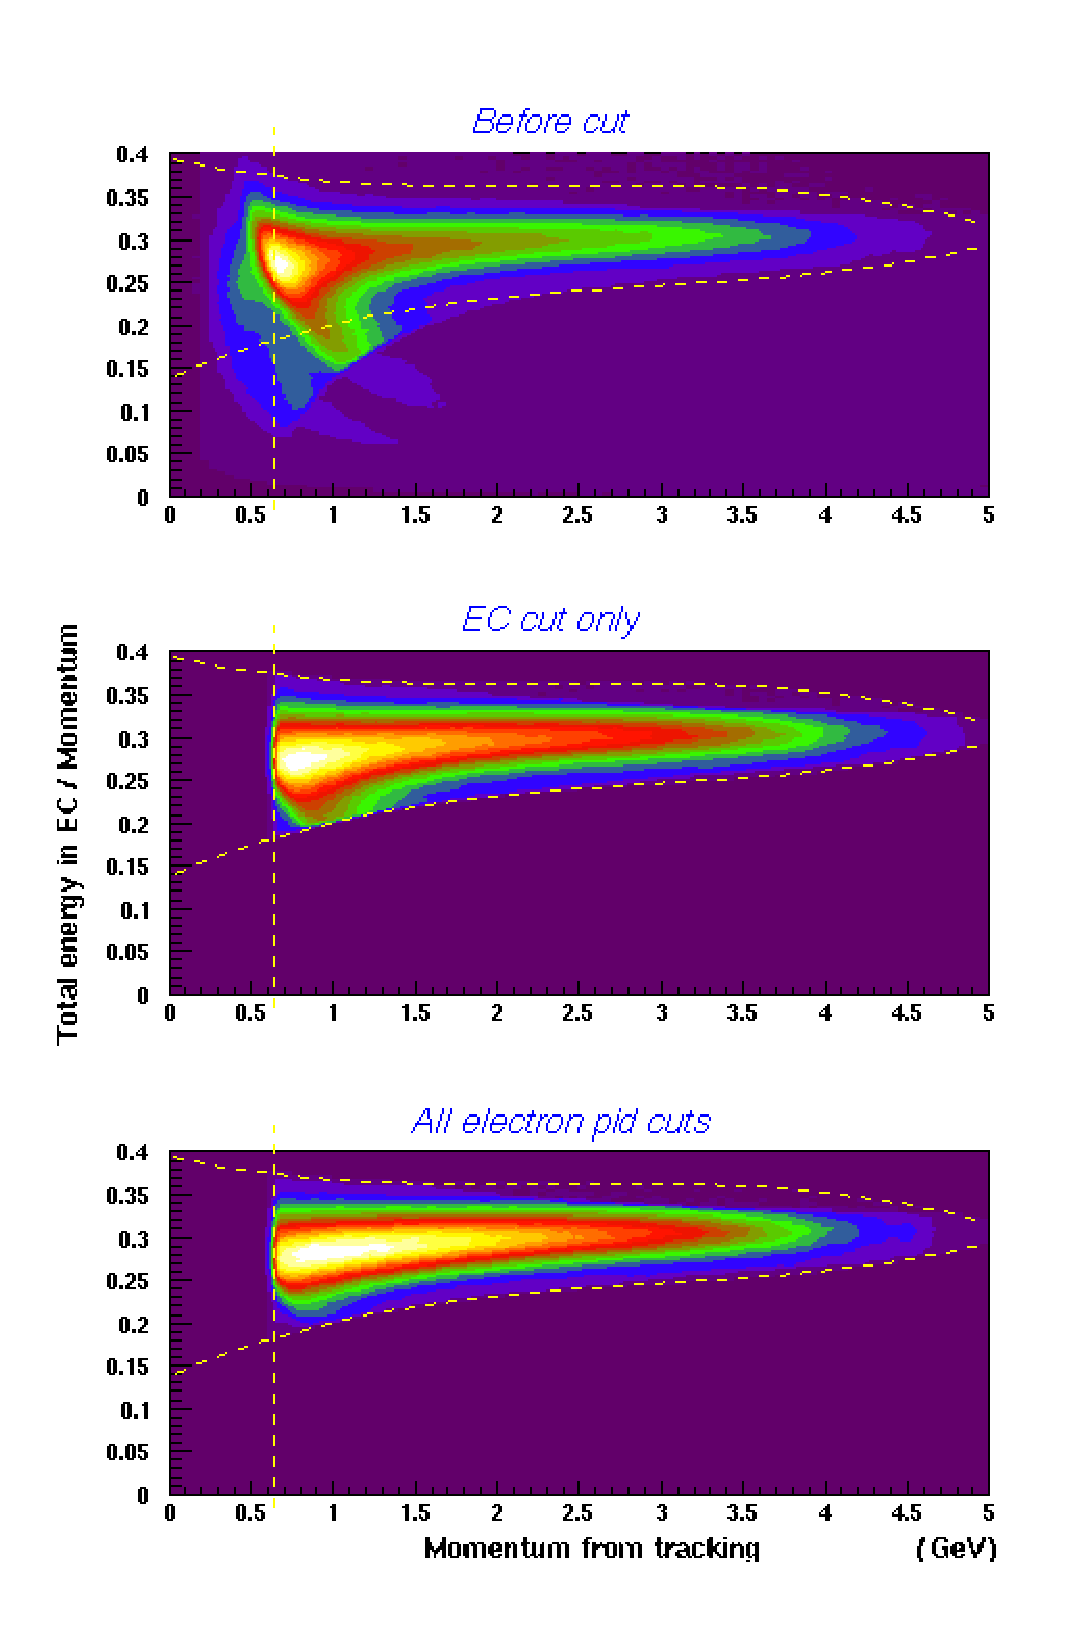
\includegraphics[width=8cm, height=11cm]{img/Ec1} 
  \caption{\cit The EC cut: the ratio $E/P$ as a function of P. 
               The vertical dashed line represents the electron momentum cut.
               The remaining two lines are the $mean$ $\pm$ $3\sigma$ cuts.
               Top plot: data without any cuts. 
               Center plot:  effect of this cut only. Events within three sigmas around the centroid of the distribution.
               Bottom plot:  all the remaining electron particle id cuts discussed are applied.}
 \label{fig:eccut}
 \end{center}
\end{figure}
\item A cut on electron momentum: a lower cut on electron momentum was applied.
This comes from a study \cite{bib:ecmin} of the inclusive cross section which gives $P_{min}$ as a function 
of EC low total threshold. The low threshold for $e1-6$ experiment was set at $172\, mV$, thus fixing
the low momentum threshold at $0.64\, GeV$. This cut is also shown in Fig.\ref{fig:eccut}.
\item A cut on the inner/outer part of the forward calorimeter: electrons release more energy in the inner part,
while pions release comparable energy in the inner/outer parts. 
\item The energy in the the inner part of the calorimeter divided by the total energy 
      in the calorimeter ($E_{in}/E_{TOT}$): the inner part is 3/8 
of the total length. Considering that electrons release more energy in the inner part, a 40\% low threshold 
cut on the ratio inner/total is introduced.
\item The track position in the EC plane: to stay away from edge effects, only tracks within 10 cm of the 
calorimeter edge are included in the analysis.
\end{itemize}

Regarding the particles identification, the mass of a track is calculated using the formula
$m^2=\Dfrac{p^2(1-\beta^2)}{\beta^2}$ where p is the momentum from tracking and $\beta$ is the particle velocity
calculated using the time of flight. The cut for the protons is $0.8 < m < 1.2$.




\subsection{Corrections.}
Due to drift chamber misalignment and uncertainties in the magnetic field, a sector dependent systematic error
on angles and momenta is introduced during software track reconstruction.
This can be mitigated by making empirical corrections.
\subsubsection{Electron and proton angle correction.}

\begin{wrapfigure}[17]{r}{9cm}
 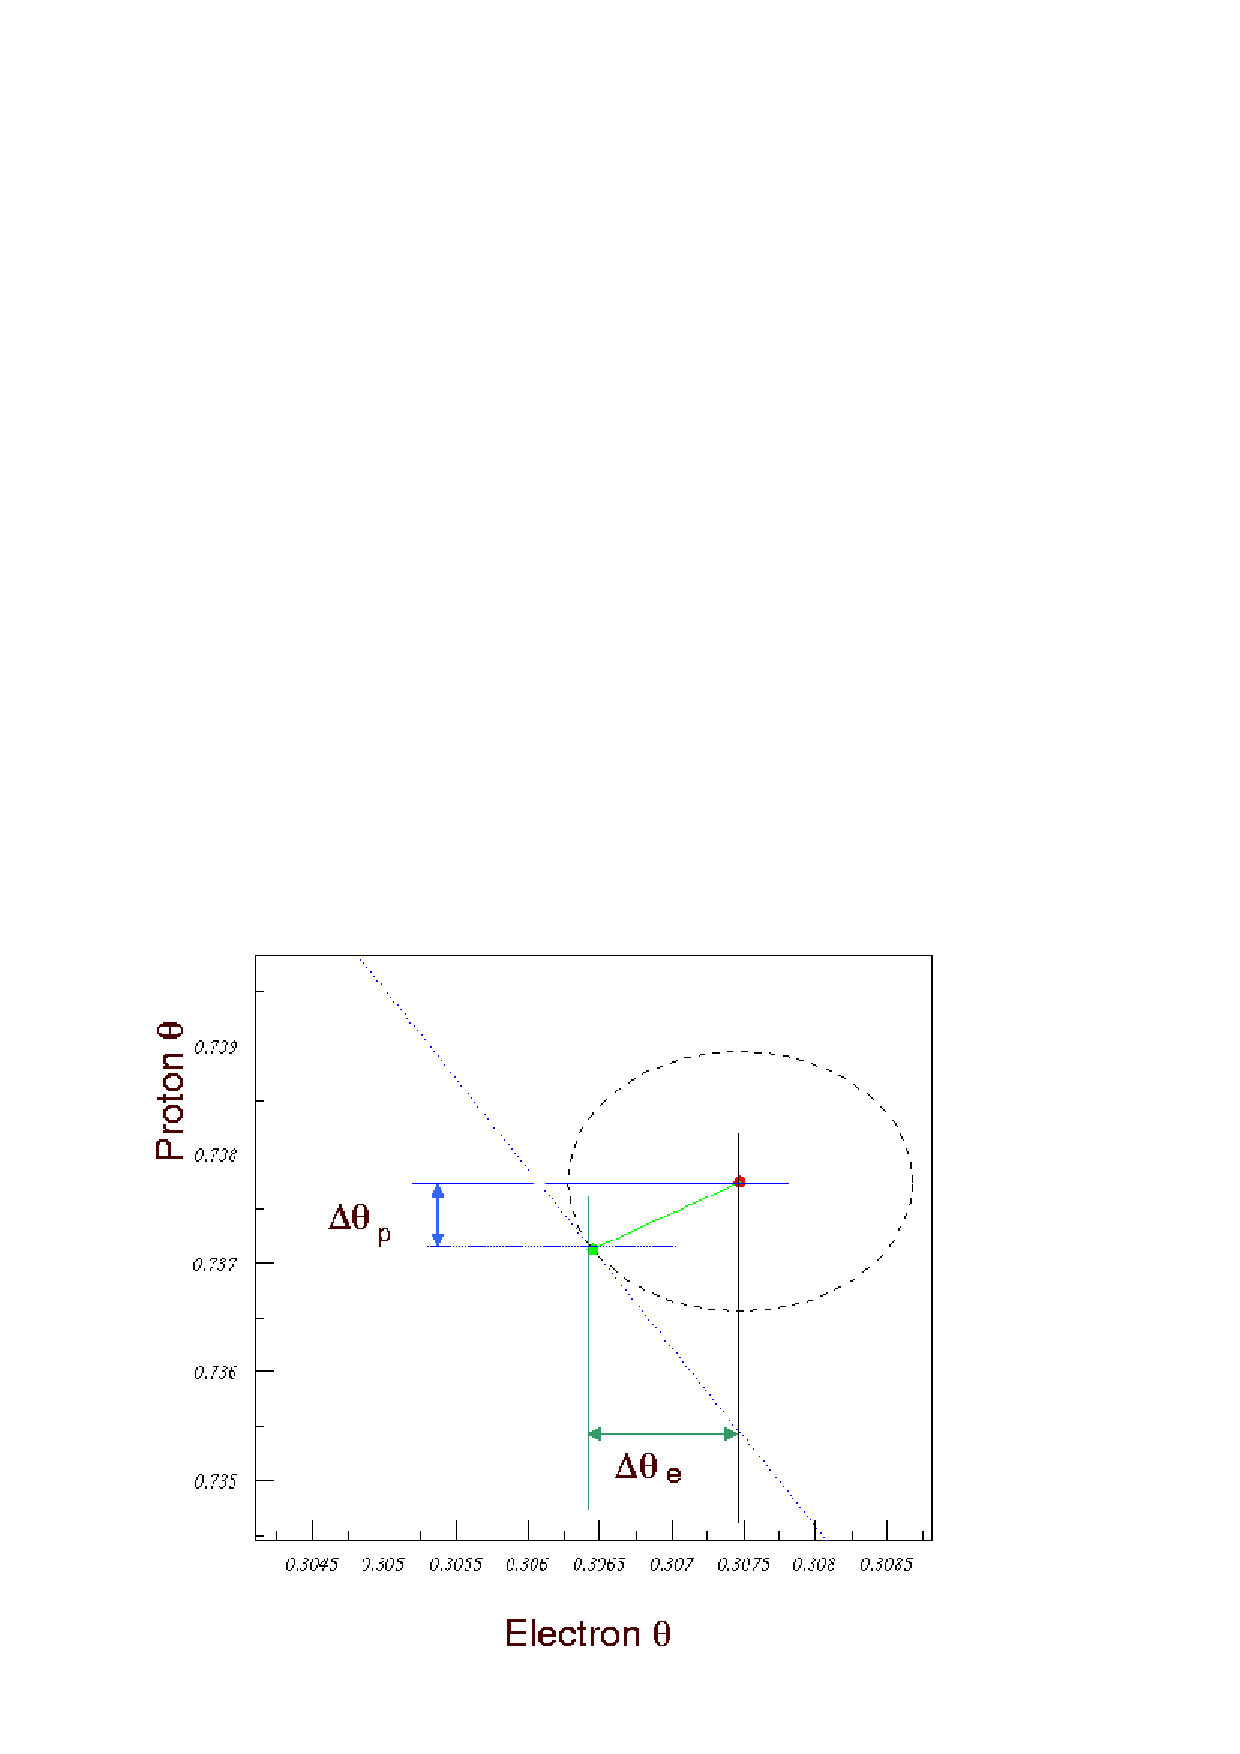
\includegraphics[width = 7.5cm, bb= 0 65 400 380]{img/closer} 
 \caption{\cit $\theta_P$ versus $\theta_e$ curve for elastic events.
              The closest point (green) of a real event (red) to this curve is found thus giving the 
              proton  and electron corrections.}
 \label{fig:closer}
\end{wrapfigure}

Assuming that the beam energy is 5.754 GeV \footnote{This comes from an independent Hall A and B study.}, 
the angles of electrons and protons 
{\bf for elastic scattering}
are correlated with the formula
$$ E = m_P-\Dfrac{m_P}{tan(\theta_e/2) tan\theta_P}  \, ,$$ 
thus giving a curve in the $\theta_P$ vs $\theta_e$ plane
as shown in Fig.\ref{fig:closer}.
On an event by event basis, the closer point to this curve is found, thus giving a distribution
of corrections $\Delta\theta_e$, $\Delta\theta_P$ which is then used for the electrons angle corrections.
The correction is at most $1\, mrad$ and it is not shown here.

\subsubsection{Electron momentum correction.}


\begin{wrapfigure}[16]{l}{9cm}
 \vspace{-1.3cm} 
  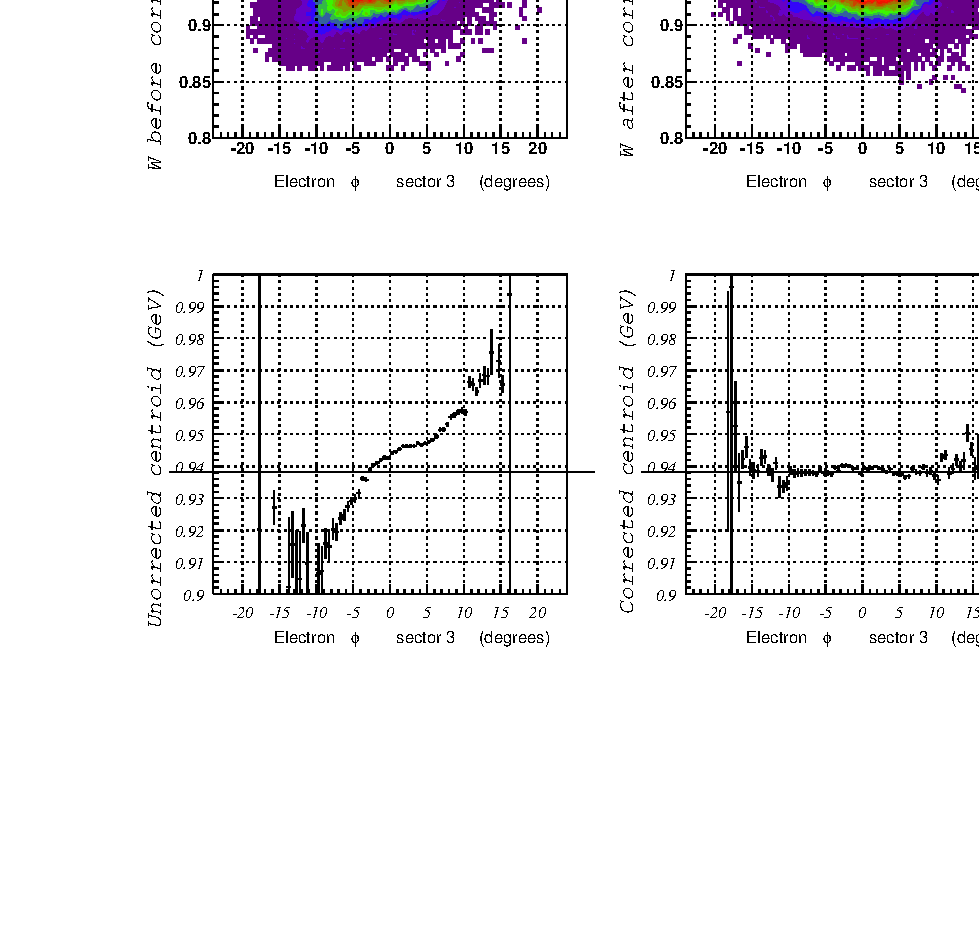
\includegraphics[height=7.8cm, bb=50 150 300 580]{img/result_pass1} 
  \caption{\cit At the top are the W distributions versus $\phi$, uncorrected (left) and corrected (right). 
               At the bottom are the centroids of the distribution before  correction (left) and after (right). 
               The horizontal line is the mass of the proton.}
 \label{fig:ecorr}
\end{wrapfigure}


Assuming that the scattered electron angle $\theta_e$ and the beam energy $E$ are correct, for all the elastic events, 
a $\Delta p=p_{calc}-p_{measured}$ is calculated using the formula
$$
 p_{calc} = \Dfrac{E}{1+\Dfrac{2Esin^2(\theta/2)}{M_P}}\, ,
$$
$M_P$ being the mass of the proton. 
Once $\Delta p$ is obtained, a function of electron $\theta$ and $\phi$ is fitted to it thus giving the correction.
The result of electron angle and momentum correction for sector three is shown in Fig.\ref{fig:ecorr}.



\newpage
\subsubsection{Proton momentum correction.} 
After correcting for the electron, a similar correction for the proton was calculated using the 
kinematics of elastic events (as above) and $\pi^0$ production as well.
We found that the correction is very small thus we didn't correct for the proton momentum.



\section{Fiducial cuts.}
In order to calculate the acceptance and to minimize CLAS inefficiencies, a fiducial volume cut is necessary
to select only trustworthy regions.
For electrons, the main problem is due to the \v Cerenkov detector inefficiency near the border of the detector. 
This reflects as a loss of statistics and inaccuracies around the edges, which is visible in all detectors because
the \v Cerenkov is in the trigger.
A volume fiducial cut for electrons based on track position is introduced. Only tracks
well within the calorimeter EC, the time of flight TOF and the \v Cerenkov CC boundaries are kept in the analysis.
Fig. \ref{fig:fidu} is an example of the cut.
\begin{figure}[h]
 \begin{center}
  \includegraphics[width=10cm, height=7cm]{img/fidu.ps} 
  \caption{\cit Fiducial volume at the plane of EC. The Y position of the tracks in EC plane versus the X position. 
                Border wiggles, due to \v Cerenkov inefficiencies, are clearly visible.}
  \label{fig:fidu}
 \end{center}
\end{figure}

\vspace{-1cm}
\section{Bethe-Heitler suppression.}
Since the $\pi^0$ is reconstructed by missing mass, there is some contamination from elastic $eP\rightarrow e'P'$ events
in which one or more real or virtual photons are produced  as illustrated in Fig.\ref{fig:bethe}. 
\begin{figure}[h]
 \begin{center}
  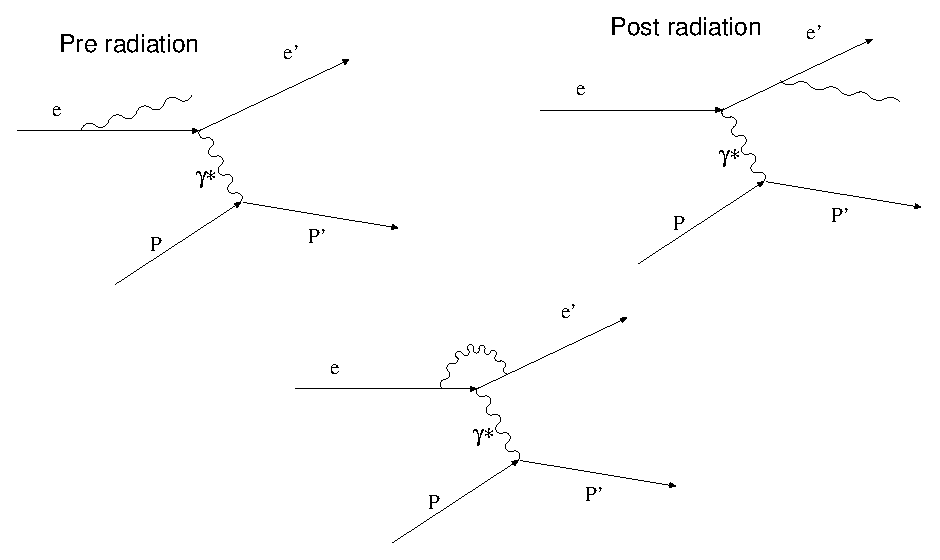
\includegraphics[height=5.5cm]{img/bethe.eps} 
  \caption{\cit Example of Bethe-Heitler processes contaminating the $\pi^0$ missing mass.}
  \label{fig:bethe}
 \end{center}
\end{figure}


The main contribution comes from
the so called pre and post radiation, in which either the beam electron or the scattered electron emits a photon. Processes
with more electromagnetic vertices are higher $\alpha$ order and therefore much less probable.

Pure elastic events are coplanar, i.e. the scattered electron and proton lie in the same plane.
When a photon is emitted the deviation from coplanarity is limited, because the angle of the photon
with respect to the incoming or scattered electron is very small, thus proton angle with respect to the scattering
plane is centered at zero with small deviations.
Fig. \ref{fig:bhcut} illustrates the cut used to eliminate Bethe-Heitler photon events from $\pi^0$ events. The angle
of the missing particle $X$ in the $\gamma^*P$ center of mass is plotted versus
the missing mass squared of the (eP) system for different W values. 
\begin{figure}[h]
 \begin{center}
  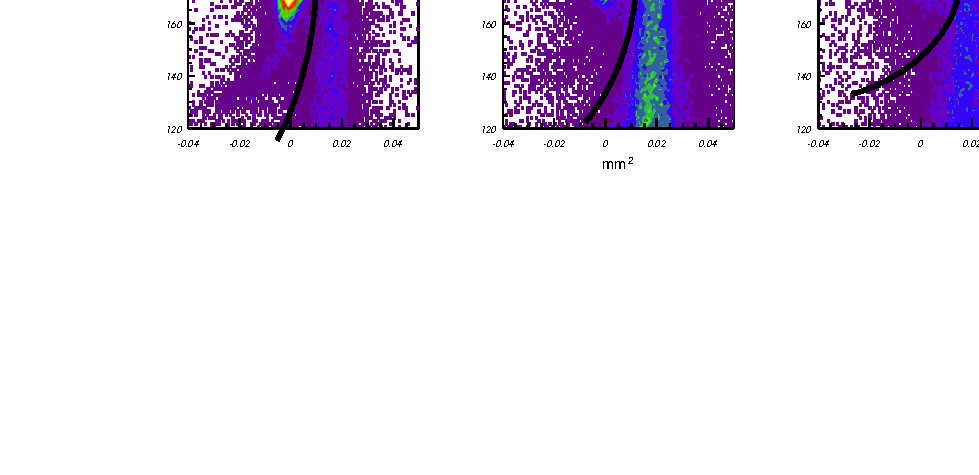
\includegraphics[height=5.7cm, bb = 230 80 220 330]{img/bethecut} 
  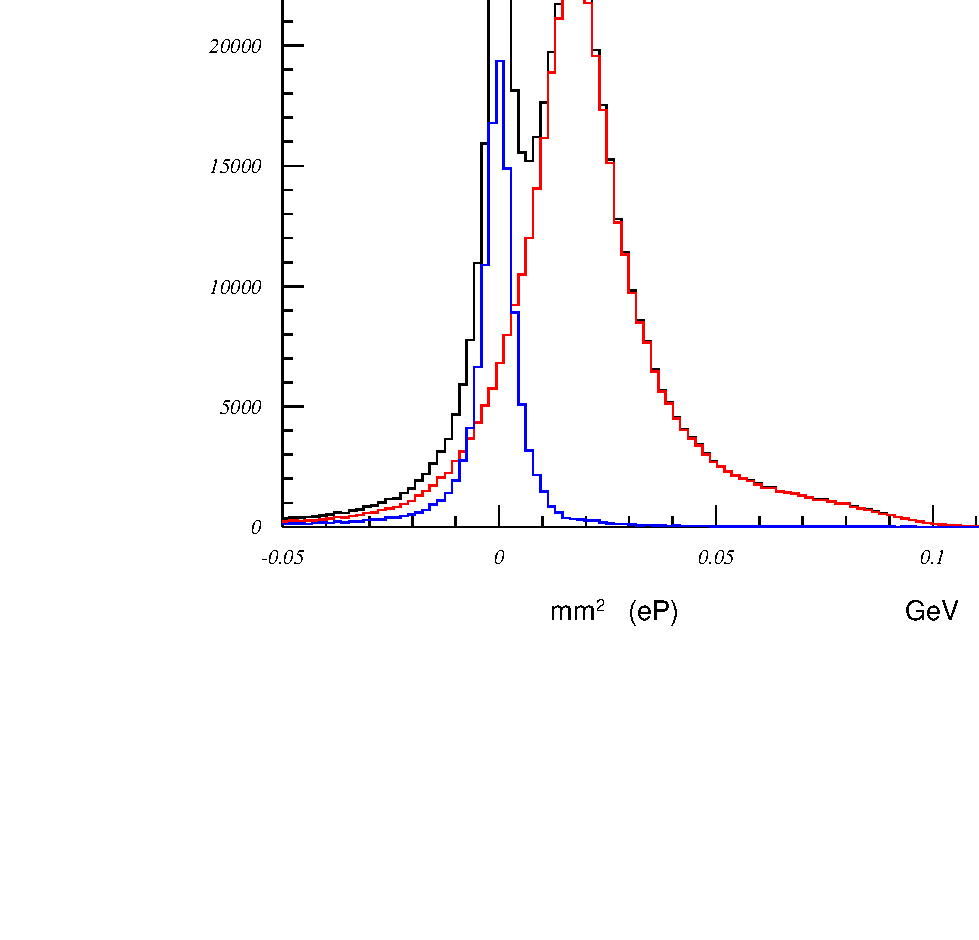
\includegraphics[height=4.7cm, bb = -420 80 220 450]{img/Allmm}
  \caption{\cit Left plots: missing angle ($\phi_{\pi_0^*}$) versus missing mass 
                $mm^2(eP)$ for different $W$ bins ($\Delta W = 50 MeV$).
                One can see the elastic radiative events concentrating on $(0,180^0)$ as well as the vertical band of $\pi^0$s. 
                As $W$ increases, the angle spread of the BH photons becomes
                smaller, but the $mm^2$ spread increases, so that a cut through the missing mass is necessary for $W = 1.35$. 
                The lost $\pi^0$s will be recovered by a Monte Carlo simulation. 
                Right plot: the $mm^2(eP)$ histogram. Photon and $\pi^0$ events are peaked around $0$ and $0.018$ 
                $GeV^2$ respectively. The black line represents all events, the red and 
                blue lines are the kept and rejected events. The $mm^2(eP)$ of $\pi^0$ is $0.0182\, GeV^2$.}
  \label{fig:bhcut}
 \end{center}
\end{figure}


\section{Radiative tail correction.}
After getting rid of elastic (radiative) processes, there is still radiative tail coming from the $\Delta(1232) $ production
which is impossible to cut off with kinematic tools. 
Mo and Tsai \cite{bib:motsai} developed a formalism to calculate the cross section and the corresponding correction. 
Afanasev, Akushevich, Burkert, and Joo produced the program {\it exclurad} to use the non approximated (i.e. without peaking approximation) Mo and Tsai formula to produce the correction for each bin in $W, Q^2, cos\theta^*, \phi^*$. 
The content of the corrected bin $B'$ is $$B' = B/C$$ where $B$ is the content of the original bin and $C$ is the 
correction.
The input models I used as exclurad input are {\it maid2000-extended} \cite{bib:maid2000} and 
{\it dmt 2001 model} \cite{bib:dmt2001}.
Fig.\ref{fig:radiation} is an example of the correction as a 
function of $\phi^*$ for $W=1.25\,GeV$ and $Q^2 = 4.75 \, GeV$.
\vspace{4cm}
\begin{figure}[h]
 \begin{center}
  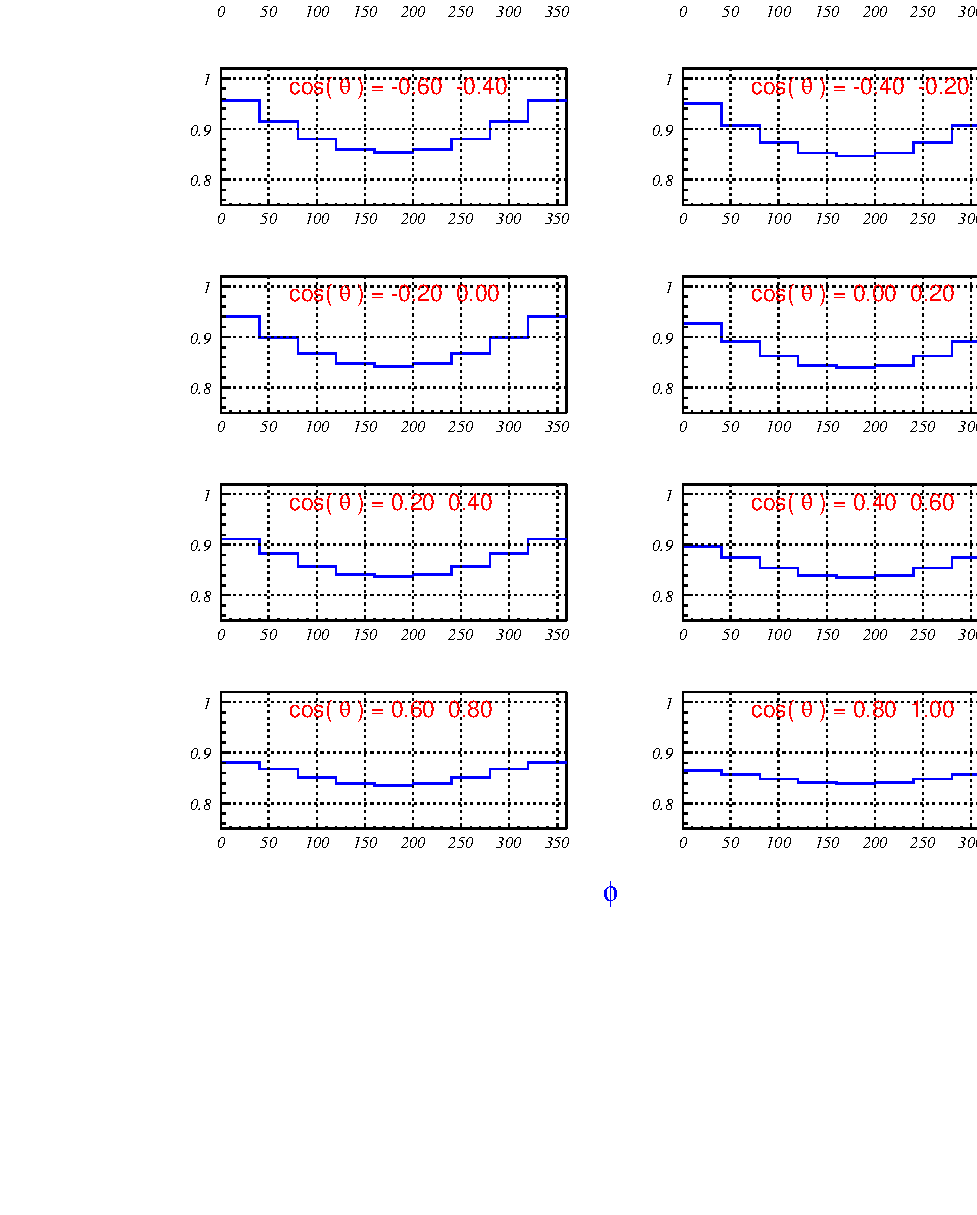
\includegraphics[width=12cm, bb=0 140 500 520]{img/radiative} 
  \caption{\cit Radiative correction as a function of $\phi_{\pi^0}^*$ for different $cos\theta^*$ bins 
                using DMT dynamical model. As seen they can be very large, comparable with the which effects we are 
                looking for.}
  \label{fig:radiation} 
 \end{center}
\end{figure}

\section{Acceptance calculation.}
The acceptance calculation has the following main goals.

\begin{itemize}
\item Normal detector acceptance: recovers limited CLAS geometrical coverage.
\item Compensates for hardware and software inefficiencies.
\item Recovers $\pi^0$ events thrown away with elastic radiative cuts. 
\item Solves bin migration problems: when an event is simulated at the vertex in a particular $W, Q^2, cos\theta^*, \phi^*$ bin,
       it can migrate to some other bin.
\end{itemize}
The Monte Carlo simulator (called GSIM) includes all major features of CLAS, but has to be corrected in order 
to make its output closer to the real data distribution using the following techniques:
\begin{itemize}
\item The Drift chamber distributions have to be smeared out. GSIM has a time to distance function
      different than the real case that leads to a resolution which is too narrow compared to the real case 
\item The Time of flight scintillator distributions have to be smeared out.
\item The drift chamber wire inefficiencies and correlations are introduced in the simulation.
      In the real data, some DC regions are defective or have low efficiency, but for GSIM all the wires
      are $100\%$ efficient. Hence inefficiencies must be introduced.
\item The time of flight dead paddles have to be removed from the simulation.
\item Since a radio frequency (RF) correction has been applied to data, the RF signal has to be simulated.
\end{itemize}
Because of bin migration, the acceptance calculation is model dependent. In fact if a certain number 
of events thrown
in one particular bin migrates to other bins, then the overall acceptance depends on the difference
in contents between one bin and another, i.e.  on the shape of the generated cross section.

The overall acceptance for a particular bin $i$ (in my case $i$ has the four index dimensions: $W$, $Q^2$,
$cos\theta^*$, $\phi^*$) is

$$ 
R_i = \Dfrac{number \,\, of\,\, events\,\, thrown\,\, in\,\, bin\,\, i}
           {number\,\, of\,\, events \,\, reconstructed\,\, in\,\, bin\,\, i}
$$


At the present moment a complete Monte Carlo simulation is not available yet.
However a first order calculation of the geometrical acceptance can be carried 
out under the assumption that in a tight enough fiducial region both the electron and proton
will {\it always} be detected.
Using cuts on the laboratory electron and proton angles as shown in Fig.\ref{fig:pseudofidu} one can generate
$\pi^0$ events\footnote{This simple model for acceptance is model independent.} 
and apply those cuts, thus generating an acceptance. 

\begin{figure}[h]
  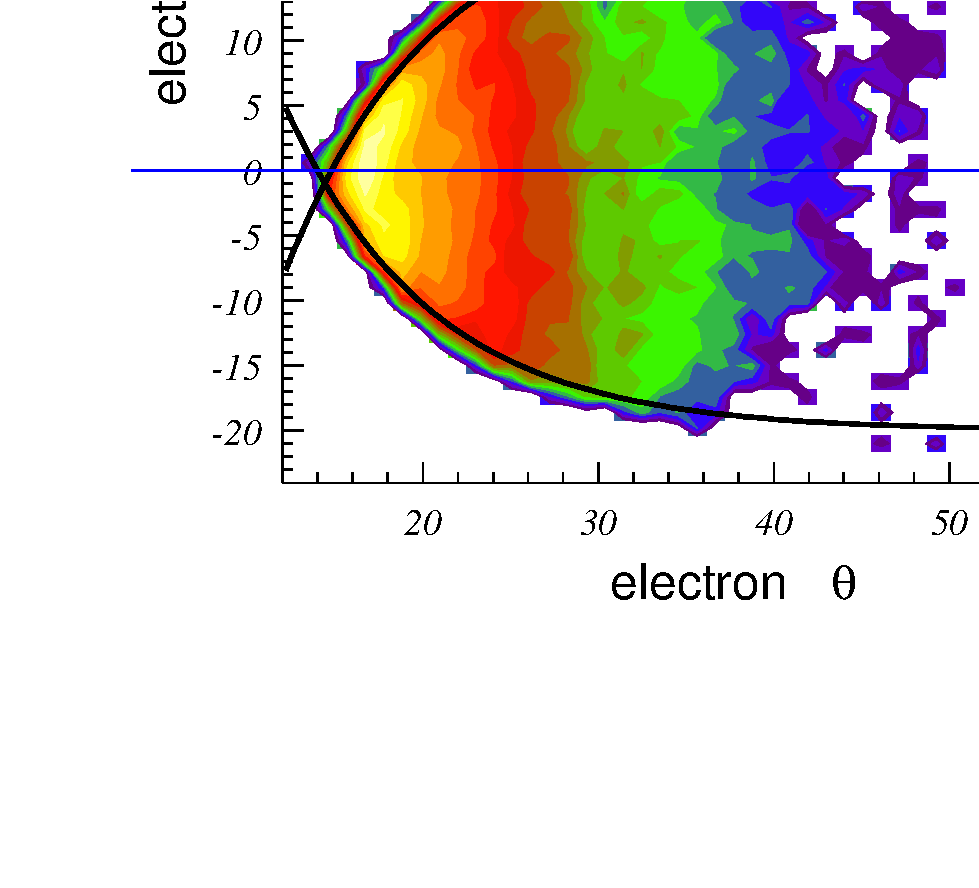
\includegraphics[height=6cm, bb = 0 100 460 500]{img/electron_pseudo} 
  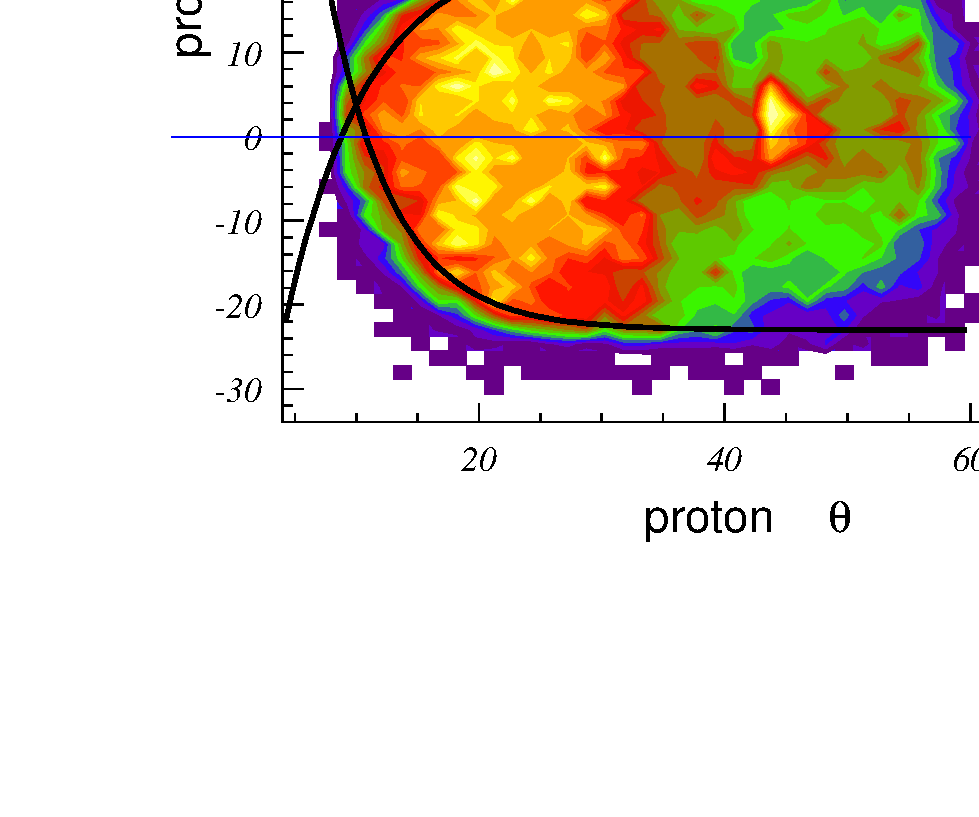
\includegraphics[height=6.5cm, bb = 0 110 200 500]{img/proton_pseudo} 
  \caption{\cit The electron (left) and proton (right) cuts on lab angles. Both particles are in sector six.
               Notice the $\phi$ asymmetries. We dont expect $\phi$ symmetry
               at fixed theta because these are $eP$ coincidence events.}
  \label{fig:pseudofidu} 
\end{figure}
The distribution of this ``pseudoacceptance'' for a particular value of $W$ and $Q^2$ is shown in Fig.\ref{fig:acce}.
\begin{figure}[h]
 \begin{center}
  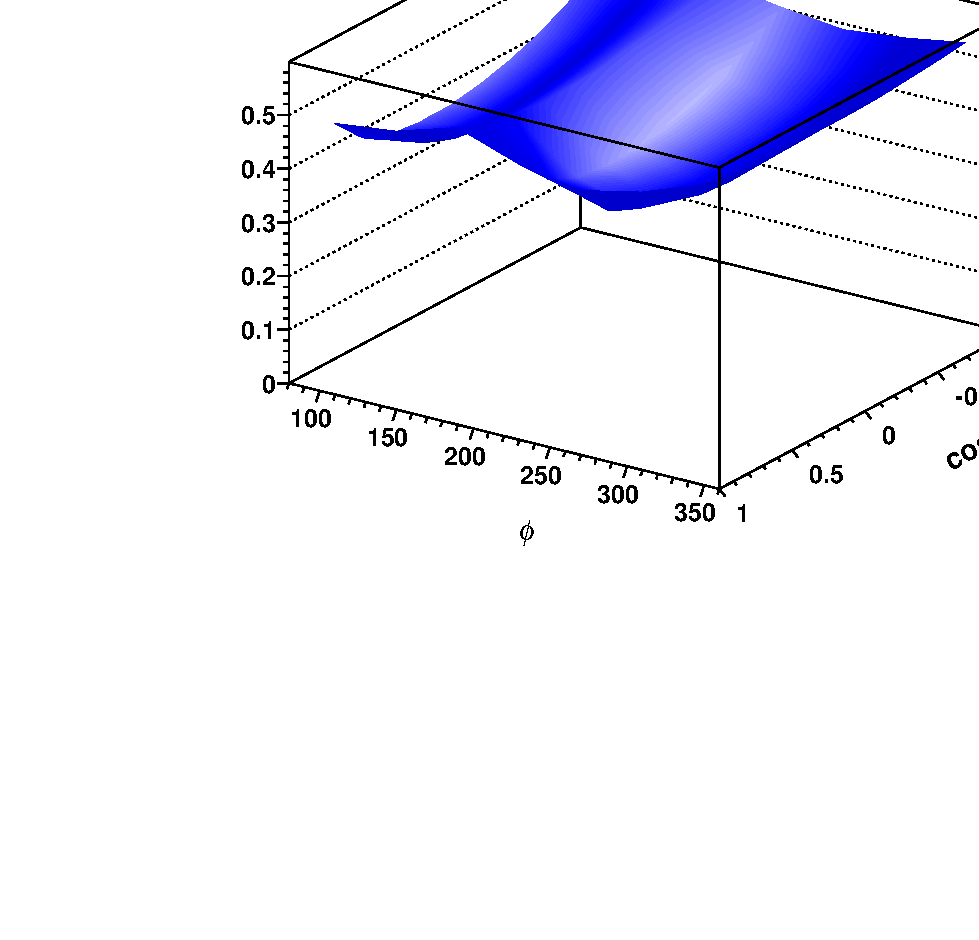
\includegraphics[height=6cm, bb = 80 200 400 540]{img/acce} 
  \caption{\cit The ``pseudoacceptance'' as a function of $\cos\theta^*$ and $\phi^*$. The $\phi^*$ deeps comes from
                the low $\phi_{lab}$ cuts, as well as their asymmetries.}
  \label{fig:acce} 
 \end{center}
\end{figure}
 


 
